\section{Arquitectura del Sistema}

Se busco encontrar una soluci�n general, siempre que fuera posible, a los problemas particulares planteados. Para ello en primer lugar se dividi� el problema principal en varios subproblemas de alcance acotado.

\subsection{M�dulos}

Se definieron entonces los siguientes m�dulos:
\begin{itemize}
\item Parser: Se encarga de la normalizaci�n del texto y extracci�n de las diferentes palabras. Es utilizado por el programa principal, pidi�ndole el listado de palabras normalizadas de un archivo.
\item AudioService: Abstracci�n de las clases de manejo de audio proporcionada por la materia. Se incluye un InputStream para proporcionar a la biblioteca de audio que facilita la serializacion de ese InputStream. Es utilizado por el programa principal para la obtenci�n y reproducci�n de audios.
\item Buffers: Permiten el intercambio de datos con los archivos, funcionando como una memoria temporal donde se acumulan los datos leidos y los que se van a escribir. Son utilizados por el FileManager como herramienta para la lectura y escritura de datos en conjunto con los serializadores. Es la herramienta de intercambio de datos entre el FileManager y los Serializadores.
\item Serializers: permiten realizar la transformaci�n de los datos hacia un tipo unificado que pueda ser almacenado en los archivos y su posterior recuperaci�n. Brinda una interfaz unificada para que el FileManager pueda realizar la conversi�n de los datos recibidos. Intercambia los datos con el FileManager mediante el uso de Buffers. Se hicieron implementaciones gen�ricas (para los datos primitivos) e implementaciones customizadas para nuestros registros que usan auxiliarmente a las gen�ricas.
\item FileManager: Manejador de archivos de registros de longitud variable en bloques. Es una implementaci�n generica que se customiza indicando el tama�o de los bloques y el serializador a usar. Permite el encadenado de bloques de manera tal que un registro serializado que exceda un bloque pueda ser guardado. Utiliza auxiliarmente a los Buffers para la acumulaci�n de datos desde y hacia los archivos y para la interacci�n con los serializadores.
\item PersistenceService: Es, principalmente, una customizaci�n (dos en realidad) del FileManager para la interacci�n con los archivos de los requerimientos; esta customizaci�n implica la definici�n de los serializadores (dos tambi�n) adecuados para los registros a usar. Adem�s provee herramientas al principal para la realizaci�n a un nivel m�s alto de las acciones con los archivos requeridas.
\end{itemize}

\begin{figure}[!htp]
	\begin{center}
		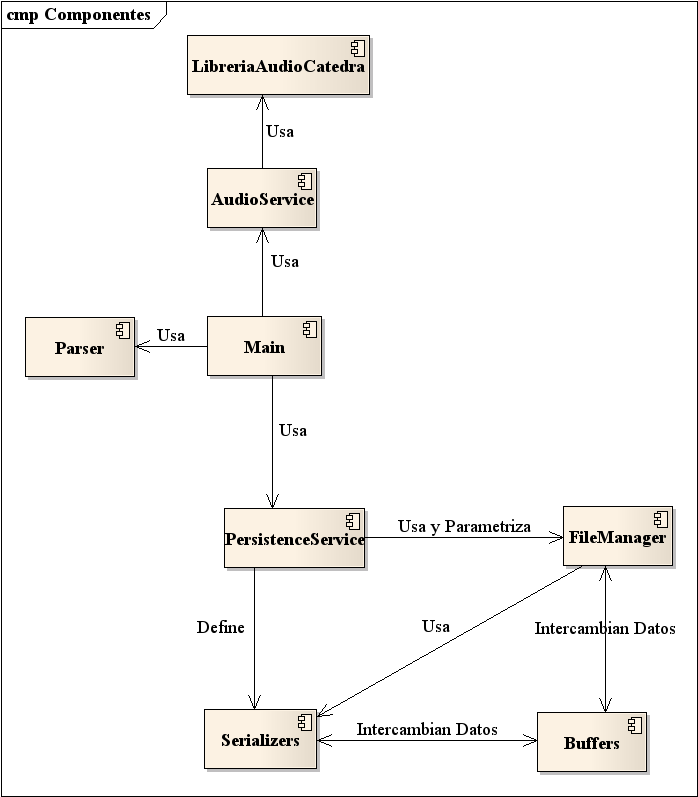
\includegraphics[scale=0.60,natwidth=512pt, natheight=163pt]{img/Componentes.png}
	\end{center}
	\caption{Diagrama de \textbf{M�dulos}} 
\end{figure}

\subsection{Definici�n de los datos}

La definici�n de los datos sigue la propuesta por los requerimientos, con la salvedad de que, dado que se usaron archivos con manejo de bloques, el offset del archivo de palabras fue dividido en dos partes; la primera indica el n�mero de bloque que almacena el sonido correspondiente; la segunda, el n�mero de objeto dentro de ese bloque.
F�sicamente, los bloques contienen informaci�n de control extra para el encadenamiento de bloques ya mencionado, pero esto se explica mejor en la secci�n correspondiente al FileManager
